% Gemini theme
% https://github.com/anishathalye/gemini

\documentclass[final]{beamer}

% ====================
% Packages
% ====================
\usepackage{fontspec}
\usepackage[T1]{fontenc}
\usepackage{lmodern}
\usepackage[size=custom,width=120,height=72,scale=1.0]{beamerposter}
\usetheme{gemini-corners}
\usecolortheme{corners}
\usepackage{graphicx}
\usepackage{booktabs}
\usepackage{tikz}
\usetikzlibrary{arrows.meta}
\usepackage{pgfplots}
\usepackage{multicol}
\setlength{\columnseprule}{1pt}

% ====================
% Lengths
% ====================

% If you have N columns, choose \sepwidth and \colwidth such that
% (N+1)*\sepwidth + N*\colwidth = \paperwidth
\newlength{\sepwidth}
\newlength{\colwidth}
\setlength{\sepwidth}{0.025\paperwidth}
\setlength{\colwidth}{0.3\paperwidth}

\newcommand{\separatorcolumn}{\begin{column}{\sepwidth}\end{column}}

% ====================
% Title
% ====================

\title{Starvation Freedom in Multi-hop Network Topologies}

\author{Rachel Wilson \inst{1} \and Pratiksha Thaker \inst{1} \and Justine Sherry \inst{1}}

\institute[shortinst]{\inst{1} Carnegie Mellon University}

% ====================
% Footer (optional)
% ====================

\footercontent{
  \href{mailto:rbwilson@andrew.cmu.edu}{rbwilson@andrew.cmu.edu} \hfill
  Meeting of the Minds, Pittsburgh --- Carnegie Mellon University \hfill
  Spring 2023}
% (can be left out to remove footer)

% ====================
% Logo (optional)
% ====================

% use this to include logos on the left and/or right side of the header:
% \logoright{\includegraphics[height=7cm]{logo1.pdf}}
% \logoleft{\includegraphics[height=7cm]{logo2.pdf}}

% ====================
% Body
% ====================

\begin{document}

\begin{frame}[t]
\begin{columns}[t]
\separatorcolumn

\begin{column}{\colwidth}

  \begin{alertblock}{Summary}

    Congestion control often uses game theory to model senders 
    competing for bandwidth in a network.
    
    In this context, prior work was able to bound conditions for bandwidth 
    starvation when senders optimize different utility functions 
    in a network with a single link.

    \textbf{This project expands that result to networks with multiple links. 
    In order to describe the utility function in these networks, 
    we model delay both deterministically and with M/M/1 queues.}
  \end{alertblock}

  \begin{block}{The Congestion Control Game}
    Senders compete for bandwith on links with given capacities.
    \begin{figure}
      \centering
      \begin{tikzpicture}
        \node [circle,draw,thick,scale=2] (link1) at (6,4) {$c_1$};
        \node [circle,draw,thick,scale=2] (link2) at (14,4) {$c_2$};
        \node [circle,draw,thick,scale=2] (linkn) at (25,4) {$c_n$};
        \node [scale=2] (s1) at (0,6) {$s_1$};
        \node [scale=2] at (0,4) {$\vdots$};
        \node [scale=2] (sn) at (0,2) {$s_i$};
        \node [scale=2] (dots) at (20,4) {$\cdots$};
        \node [scale=2] (sn1) at (10,8) {$s_{i+1}$};
        \node [scale=2] (sn2) at (21,8) {$s_{k}$};
        \draw[-{Stealth[length=6mm,width=4mm]},semithick] (s1.east) -- (link1.west);
        \draw[-{Stealth[length=6mm,width=4mm]},semithick] (sn.east) -- (link1.west);
        \draw[-{Stealth[length=6mm,width=4mm]},semithick] (link1.east) -- (link2.west);
        \draw[-{Stealth[length=6mm,width=4mm]},semithick] (link2.east) -- (dots.west);
        \draw[-{Stealth[length=6mm,width=4mm]},semithick] (dots.east) -- (linkn.west);
        \draw[-{Stealth[length=6mm,width=4mm]},semithick] (linkn.east) -- (28,4);
        \draw[-{Stealth[length=6mm,width=4mm]},semithick] (sn1.south) -- (link2.west);
        \draw[-{Stealth[length=6mm,width=4mm]},semithick] (sn2.south) -- (linkn.west);
        \end{tikzpicture}
      \caption{Multi-hop Network with Multiple Senders}
    \end{figure}

    \heading{The Utility Function}
    Sender $i$ optimizes $u_i$ as a function of its sending rate $s_i$ and the
    aggregate load $Q$
    
    {\Large\[u_i(s_i, Q) = T(s_i, Q) - \alpha_i s_i D(s_i, Q) \]}

    Each sender is rewarded for throughput, determined by $T$, and penalized for
     delay, given by $D$, which is scaled by a delay sensitivity parameter $\alpha$.
  \end{block}

  \begin{block}{Goal}
    \begin{Large}
      
      \textbf{To model delay in multi-hop networks in two ways.}
      \begin{enumerate}
        \item Reasoning deterministically for a single sender
        \item Using Poisson processes for arbitrary senders
      \end{enumerate}
    \end{Large}

  \end{block}

\end{column}

\separatorcolumn

\begin{column}{\colwidth}

  \begin{block}{Deterministic Delay with One Sender across Multiple Links}
    \begin{figure}
      \centering
      \begin{tikzpicture}
        \node [circle,draw,thick,scale=2] (link1) at (6,4) {$c_1$};
        \node [circle,draw,thick,scale=2] (link2) at (11,4) {$c_2$};
        \node [circle,draw,thick,scale=2] (linkk) at (21,4) {$c_n$};
        \node [scale=2] (s1) at (0,4) {$s_0$};
        \node [scale=2] (dots) at (16,4) {$\cdots$};
        \draw[-{Stealth[length=6mm,width=4mm]},semithick] (s1.east) -- (link1.west);
        \draw[-{Stealth[length=6mm,width=4mm]},semithick] (link1.east) -- (link2.west);
        \draw[-{Stealth[length=6mm,width=4mm]},semithick] (link2.east) -- (dots.west);
        \draw[-{Stealth[length=6mm,width=4mm]},semithick] (dots.east) -- (linkk.west);
        \draw[-{Stealth[length=6mm,width=4mm]},semithick] (linkk.east) -- (25,4);
        \end{tikzpicture}
      \caption{One sender into an arbitrarily long sequence of links.}
    \end{figure}
      
    \begin{center}
      \begin{tabular}{| c | l |}
        \hline
        $p$ & \# of packets\\
        \hline
        $b$ & \# of bits per packet\\
        \hline
        $c_i$ & capacity of link $i$\\
        \hline
      \end{tabular} \ \ \ \
      \begin{tabular}{| c | l |}
        \hline
        $c_\mathrm{min}$ & smallest of all link capacities\\
        \hline
        $w_i$ & idle time per packet on link $i$\\
        \hline
        $s_0$ & initial pace set by the sender\\
        \hline
      \end{tabular}
    \end{center}
    
    {\large
    \[\textbf{end-to-end time for $p$ packets} = \frac{pb}{c_\mathrm{min}} + \sum_{i\neq \mathrm{min}}^{n}\frac{b}{c_i}\]}\\
    First term: Time per packet on the slowest link\\
    Second term: Time it takes the first packet to traverse all links
  \end{block}
  \begin{exampleblock}{Proof Sketch}
      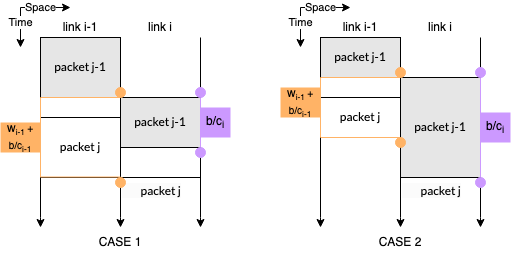
\includegraphics[scale=2]{Cases.png}
  
    {\Large Between two arbitrary links, we observe how packet spacing changes.
    \begin{itemize}
      \item \textbf{Case 1:} $\frac{b}{c_{i-1}} + w_{i-1} \geq \frac{b}{c_{i}} \to$ 
      Packet spacing does not change.
      \item \textbf{Case 2:} $\frac{b}{c_{i-1}} + w_{i-1} < \frac{b}{c_{i}} \to$ 
      Packet spacing increases to $\frac{b}{c_i}$.
    \end{itemize}}

    {\Large\textbf{The slowest link determines overall packet spacing.}}
  \end{exampleblock}
  \vspace{-10mm}

  
\end{column}

\separatorcolumn

\begin{column}{\colwidth}

  \begin{block}{Deterministic Drawback}
   
    When multiple senders enter the network, it is hard to reason deterministically 
    about the interleaving of packets from different senders. 
    Instead we use Poisson processes.
    
  \end{block}

  \begin{block}{Delay using Poisson Processes across Multiple Links}
    \begin{figure}
      \centering
      \begin{tikzpicture}
        \node [circle,draw,thick,scale=2] (link1) at (6,2) {$c_1$};
        \node [circle,draw,thick,scale=2] (link2) at (14,2) {$c_2$};
        \node [scale=2] (s1) at (0,4) {$s_1$};
        \node [scale=2] (s3) at (10,5) {$s_{3}$};
        \node [scale=2] (s2) at (0,0) {$s_{2}$};
        \draw[-{Stealth[length=6mm,width=4mm]},semithick] (s1.east) -- (link1.west);
        \draw[-{Stealth[length=6mm,width=4mm]},semithick] (s2.east) -- (link1.west);
        \draw[-{Stealth[length=6mm,width=4mm]},semithick] (link1.east) -- (link2.west);
        \draw[-{Stealth[length=6mm,width=4mm]},semithick] (link2.east) -- (18,2);
        \draw[-{Stealth[length=6mm,width=4mm]},semithick] (s3.south) -- (link2.west);
      \end{tikzpicture}
      \caption{A simple network with multiple senders.}
    \end{figure}

    \heading{Poisson Process}
    Sending rates $s_i$ and service rates $c_i$ are random and memoryless, as are
    departures from any link[CITE Mor].

    Merge two Poisson processes by adding their sending rates.

    \heading{Average Delay}
    $T_{s_i}$ is the average time a packet from $s_i$ spends in the Network[CITE Mor]
    {\large\begin{align*}
      \mathbb{E}[T_{s_1}] = \mathbb{E}[T_{s_2}] &= \frac{1}{c_1 - (s_1+s_2)} + \frac{1}{c_2 - (s_1 + s_2+s_3)}\\
      \mathbb{E}[T_{s_3}] &= \frac{1}{c_2 - (s_1 + s_2+s_3)}
    \end{align*}}
  \end{block}

  \begin{exampleblock}{Considerations}
    \begin{itemize}
      \item Is a Poisson model realistic?
      \item Can we make the delay aggregative with an upper bound?
      \item How can we circumvent the stability requirement for the Poisson model?
    \end{itemize}
  \end{exampleblock}
  \vspace{-10mm}

  \begin{block}{Moving Forward}
    After calculating delay, we need to make the game aggregative and revisit
    premises involving concavity in order to apply prior results
    which bound starvation.
  \end{block}

  \begin{block}{References}

    \nocite{*}
    \footnotesize{\bibliographystyle{plain}\bibliography{poster}}

  \end{block}

\end{column}

\separatorcolumn
\end{columns}
\end{frame}

\end{document}
